\section{Photomultiplier Tubes}
\label{sec:pmts}
The ID PMTs are 20-inch PMTs (Hamamatsu R3600) built by Hamamatsu Photonics K.K.  A schematic is shown in \cref{fig:pmt}  These PMTs were based off an earlier Hamamtsu designed 20-inch PMT (Hamamatsu R1449) which had been used in the Kamiokande Detector.  The Kamiokande design was improved upon in collaboration with Hamamatsu for use in Super-Kamiokande \cite{Suzuki:1992as}.  The photocathode is made of bialkali, which was chosen for its high sensitivity to blue light and low thermionic emission.  The quantum efficiency of the photocathode peaks around 21\% between 360 and 400 nm, and is shown as a function of wavelength along with the emitted spectrum of Cherenkov light in water in \cref{fig:pmt_qe_cherenkov_spectrum}. The dynode structure is a venitian blind type, which was optimized to improve photoelectron (p.e.) timing resolution and collection efficiency \cite{Suzuki:1992as}.  The single p.e. pulse height distribution and transit time distribution are shown in \cref{fig:pmt_pe_and_timing}.\par    

\begin{figure}
\centering
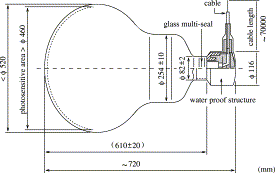
\includegraphics[width=0.8\textwidth]{figures/pmt.png}
\caption{Schematic of the ID PMTs. \cite{Fukuda:2002uc}}
\label{fig:pmt}
\end{figure}

\begin{figure}
\centering
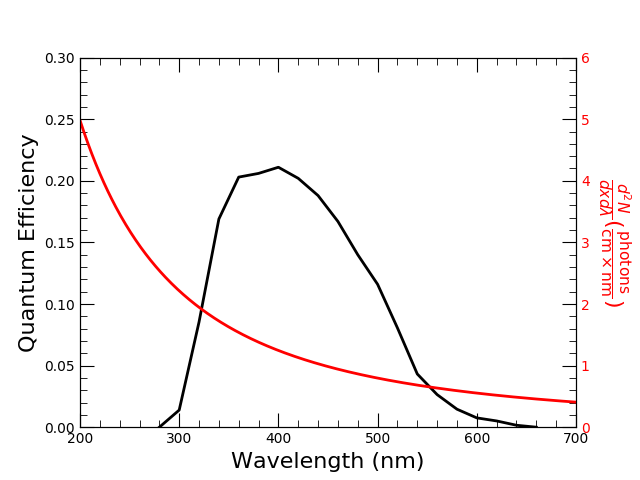
\includegraphics[width=0.8\textwidth]{figures/pmt_qe_cherenkov_spectrum.png}
\caption{Photocathode quantum efficiency in black and emitted Cherenkov spectrum in red.  Note different y-axes.}
\label{fig:pmt_qe_cherenkov_spectrum}
\end{figure}

\begin{figure}
\centering
\subfigure[]{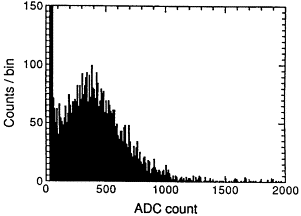
\includegraphics[width=0.4\textwidth]{figures/pmt_single_pe.png}
\label{fig:pmt_1pe_pusle_height}	
}
\subfigure[]{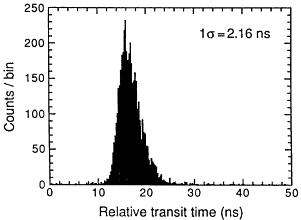
\includegraphics[width=0.4\textwidth]{figures/pmt_transit_time.png}
\label{fig:pmt_transit_time}	
}
\caption{Left: ID PMT single p.e. pulse height distribution.  The peak near zero ADC counts is the result of dark current.  Right: ID PMT relative transit time distribution at 410 nm and single p.e. level.  Both from \cite{Fukuda:2002uc}}
\label{fig:pmt_pe_and_timing}
\end{figure}

In order to prevent another accident like the one which occurred during upgrade work after SK-I, all PMTs have been enclosed in a protective case since the beginning of SK-II.  These protective cases consist of an acrylic dome over the face of the PMT, and a fiber-reinforced plastic (FRP) case around the sides and back of the PMT.  The FRP case has holes in it which allow water to flow freely around the PMT, but also restrict the speed with which water can rush into the vacuum of a PMT in case of a PMT implosion.  This mitigates the creation of a shock wave, which was determined to be the cause of the original accident.  \par

The OD PMTs are 8-inch PMTs, also produced by Hamamatsu.  Five-hundred ninety-one are old Hamamatsu R1408 PMTs, recycled form the IMB experiment, which 1293 are new Hamamatsu R5912 PMTs, installed during the upgrades between SK-I and SK-II, and SK-II and SK-III.  The single p.e. distributions for the old and new tubes are shown in \cref{fig:od_1pe}.

\begin{figure}
\centering
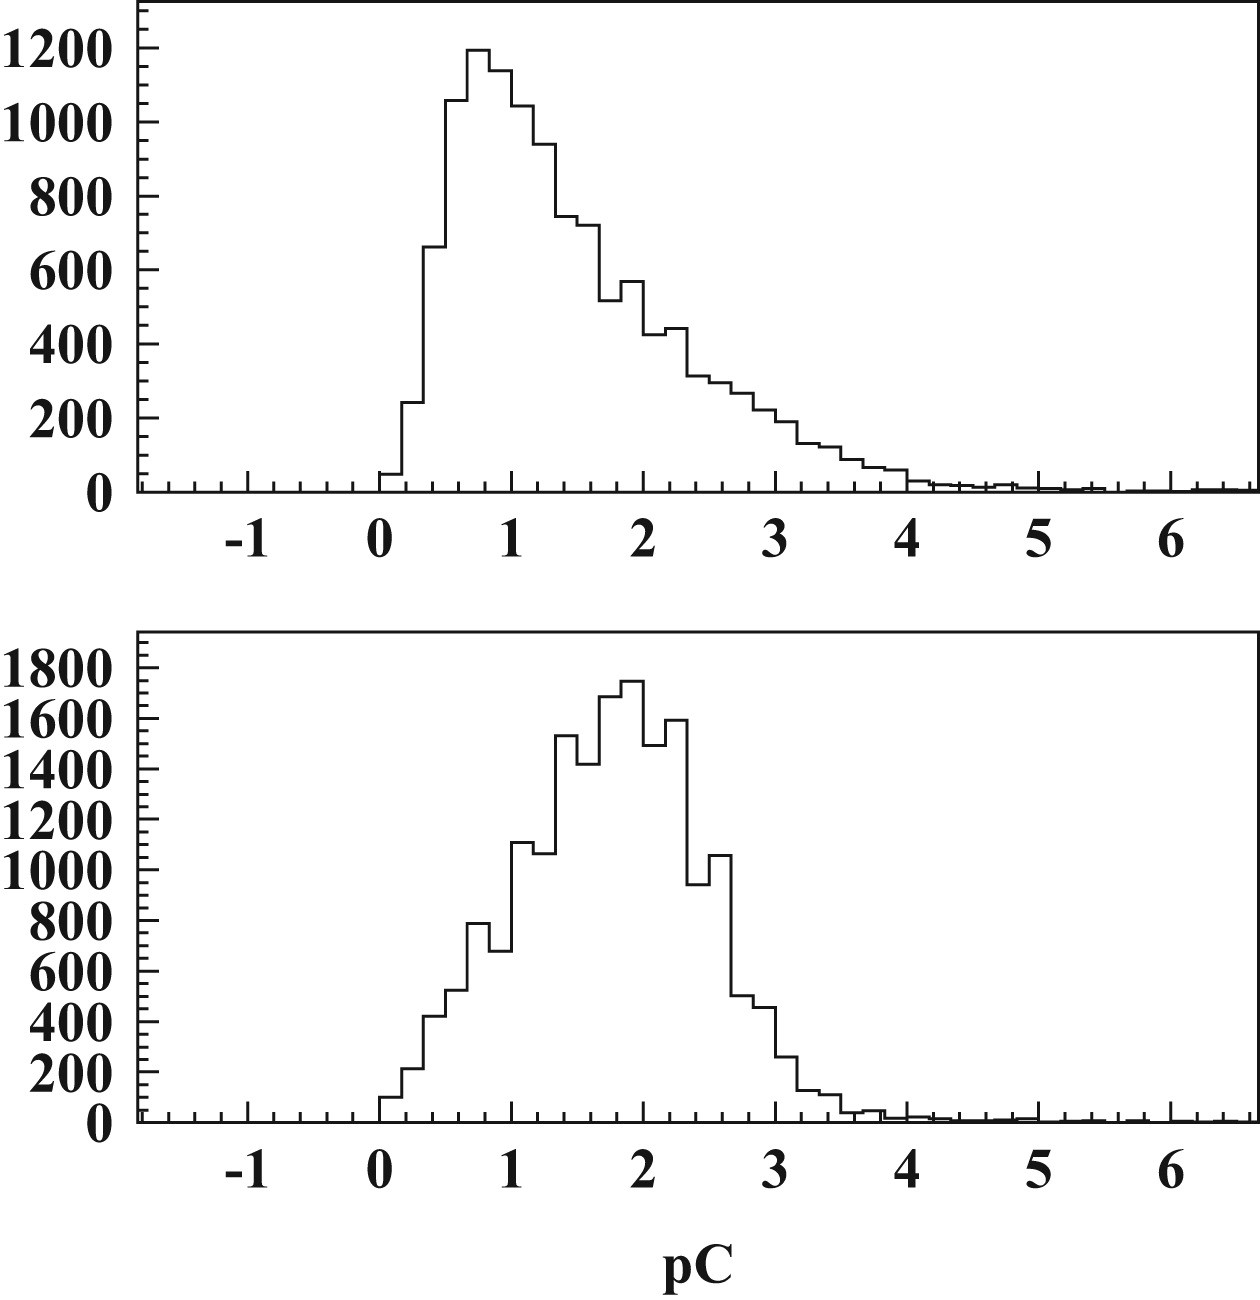
\includegraphics{figures/OD_1pe_distribution.jpg}
\caption{Top: Single p.e. distribution of OD old PMTs (Top) and new PMTs (Bottom). Both from \cite{Abe:2013gga}}
\label{fig:od_1pe}
\end{figure}
 